
\chapter{CHALLENGES}

\section{Zooko's Triangle}
\label{sec:ZookosTriangle}

Our primary objective with OnioNS is to provide human-meaningful domain names Tor hidden services, but we list distributed and securely unique domain names in our design requirements. Achieving all three objectives is not easy; a naming scheme can use a central root zone or authority to ensure that meaningful domains remain unique, but then it is not distributed; it can achieve a distributed nature by generating domain names with cryptographic hash function, but then domains are no longer human-meaningful; or it can allow peers to provide meaningful names to each other, but then these names are not guaranteed to be globally unique. This problem is illustrated in Figure \ref{fig:ZookosTriangle} and summarized by Zooko's Triangle, a conjecture proposed by Zooko Wilcox-O'Hearn in 2001. The conjecture states a persistent naming system can achieve at most two of these properties: it can provide unique and meaningful names but not be distributed, it can be distributed and provide unique names that are not meaningful, or it can be distributed and provide meaningful names that are not guaranteed to be unique\cite{ferdous2009security}\cite{stiegler2005petname}.

\begin{figure}[htbp]
	\centering
	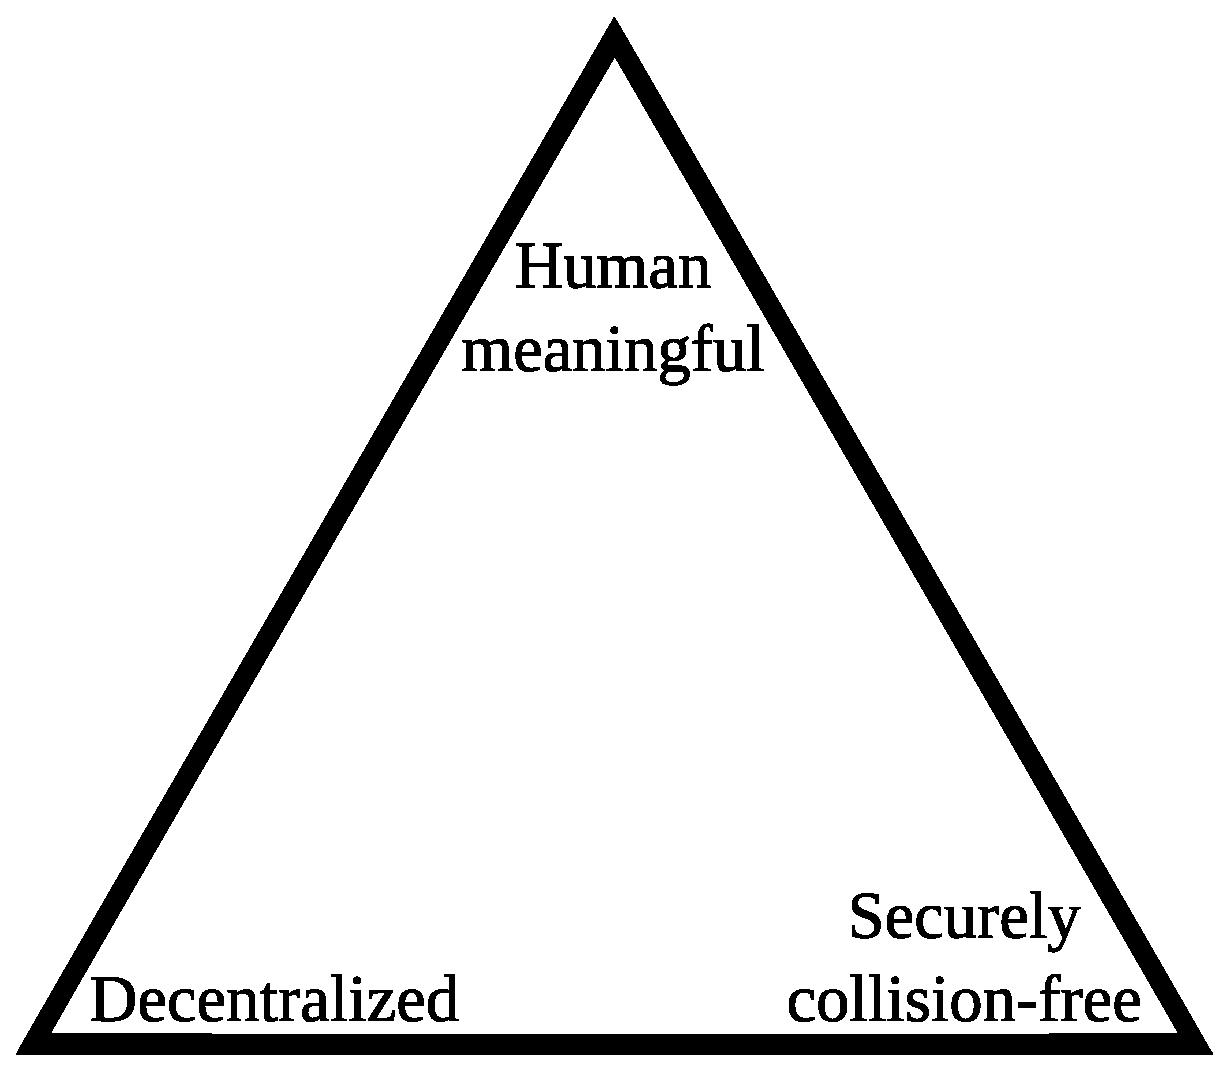
\includegraphics[width=0.4\textwidth]{images/Zooko.eps}
	\caption{Zooko's Triangle.}
	\label{fig:ZookosTriangle}
\end{figure}

Some examples of naming systems that achieve only two of these properties include:

\begin{itemize}
	\item \textbf{Securely unique and human-meaningful} --- Internet domain names are memorable and provably collision free, but the Internet DNS with a hierarchical structure with central authorities under the jurisdiction of ICANN.
	\item \textbf{Decentralized and human-meaningful} --- Human names and nicknames are legal and social labels for each other, but we provide no protection against name collisions.
	\item \textbf{Securely unique and decentralized} --- Tor hidden service .onion addresses, PGP keys, and Bitcoin/Namecoin addresses use the large key-space and the collision-free properties of cryptographic hash algorithms to ensure uniqueness, but do not use meaningful names.
\end{itemize}

\section{Non-existence Verification}

In our design requirements we specify that clients of a naming system should be able to verify the authenticity of domain names. On the Internet, the former is addressed by SSL certificates and a chain of trust to root Certificate Authorities, while the latter remains a possible attack vector. Of equal importance, however, is the capability to verify a claim of non-existence by a name server. This is a weakness often overlooked in other DNSs and resolving this problem is not easy. While DNSSEC does provide an extension for this purpose, DNSSEC has not seen widespread use and to our knowledge no alternative DNS provides mechanisms for authenticated denial-of-existence.
